\documentclass[10pt]{article}
\usepackage{amsmath}
\usepackage{amsfonts}
\usepackage{amssymb}
\usepackage{mathtools}
\usepackage{color,soul}
\usepackage{fullpage}
\usepackage{enumerate}
\usepackage{graphicx}
\usepackage{caption}
\usepackage{subcaption}
\usepackage[colorlinks=true,urlcolor=blue,breaklinks]{hyperref}

\definecolor{Light}{gray}{.90}
\sethlcolor{Light}

\title{Horizon Sun Sensor}
\author{Jeren Suzuki}
\date{Last Edited \today}

\begin{document}

\maketitle
\pagenumbering{Roman}
\tableofcontents
\newpage
\pagenumbering{arabic}

\section{Goals}
With a composite image of two Earth limbs, calcualte the ``pitch'' and ``roll'' of the camera. 

\section{Assumptions} % (fold)
\label{sec:assumptions}
I assume that the Earth's limb looks very linear and that for any given axis which the Earth seems to be flipped around, there is an Earth pixel in the perpendicular axis. This corresponds to the camera not swinging so much that half of the image is dominated by space. I also assume that the limb, even though it looks mostly linear, is an arc of a quadratic curve. 
% section assumptions (end)


\section{Starting Image} % (fold)
\label{sec:starting_image}

\begin{figure}[!h]
    \centering
    % 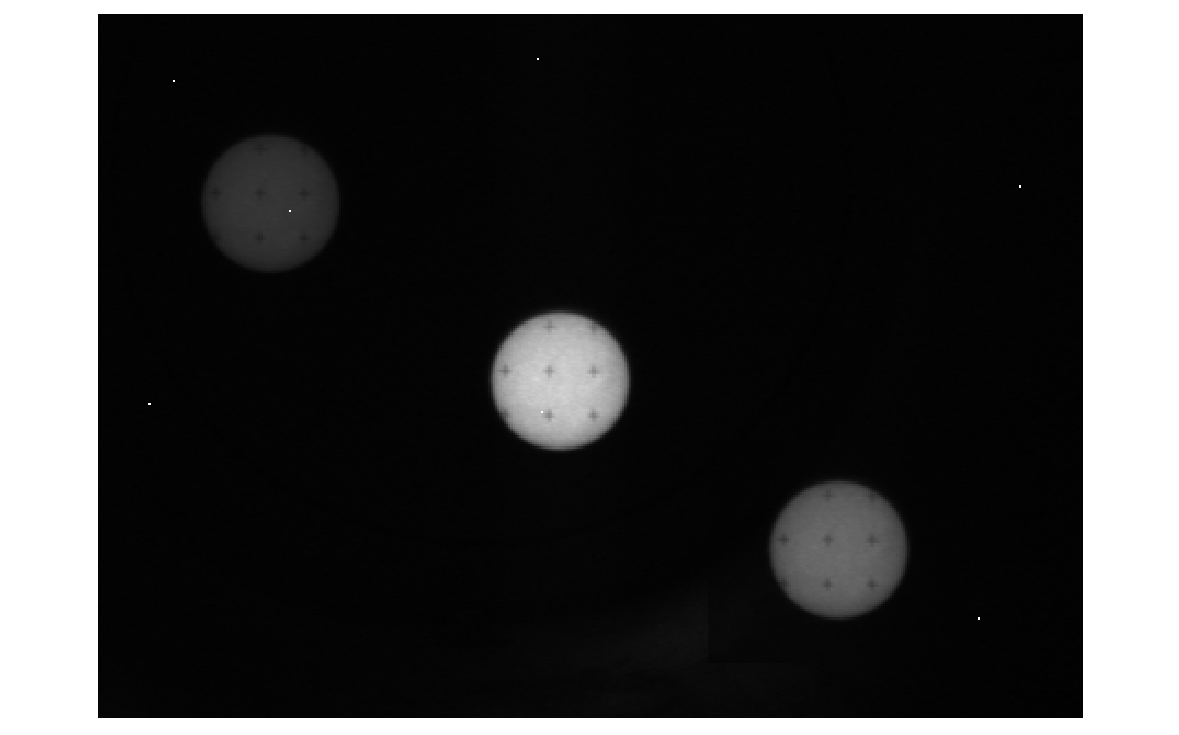
\includegraphics[width=.9\textwidth]{plots_tables_images/raw.eps}   notilt 
    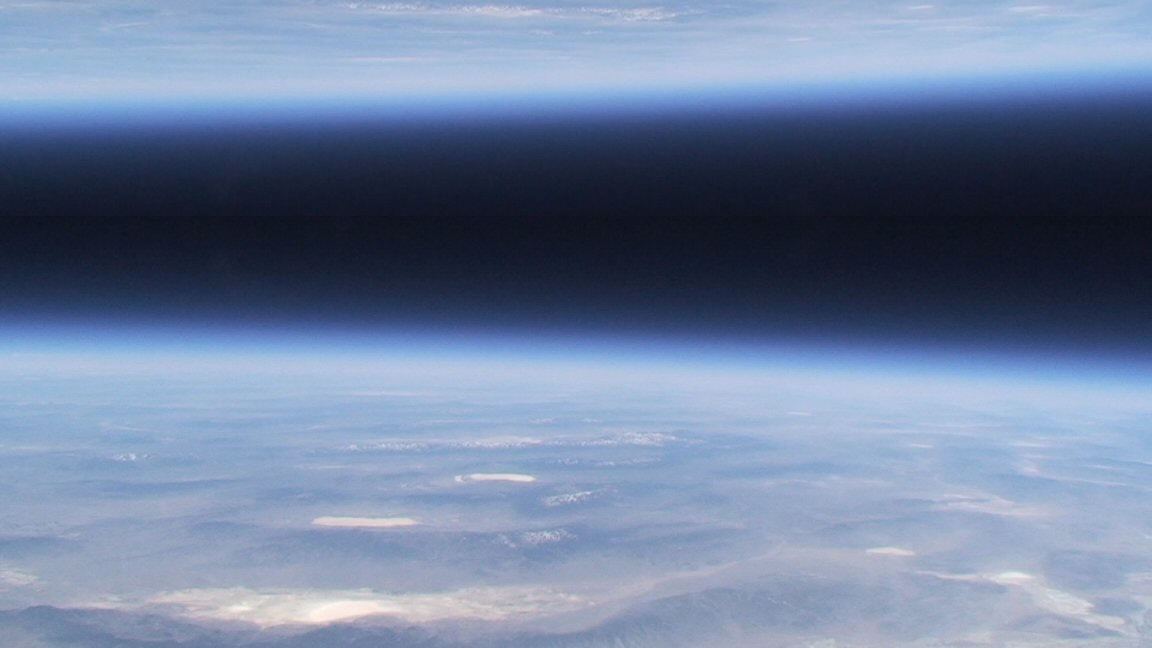
\includegraphics[width=.9\textwidth]{plots_tables_images/100kft/notilt}
    \label{raw}
\end{figure}

We will have a B/W camera using a red filter on the lens so that we will only use the red light.
% section starting_image (end)

\newpage

\section{Image Processing} % (fold)
\label{sec:image_processing}

\subsection{``Pitch''} % (fold)
\label{sub:pitch}

A threshold is set to mask the Earth in the photo, as shown in Figure \ref{rmask}.

\begin{figure}[!h]
    \centering
    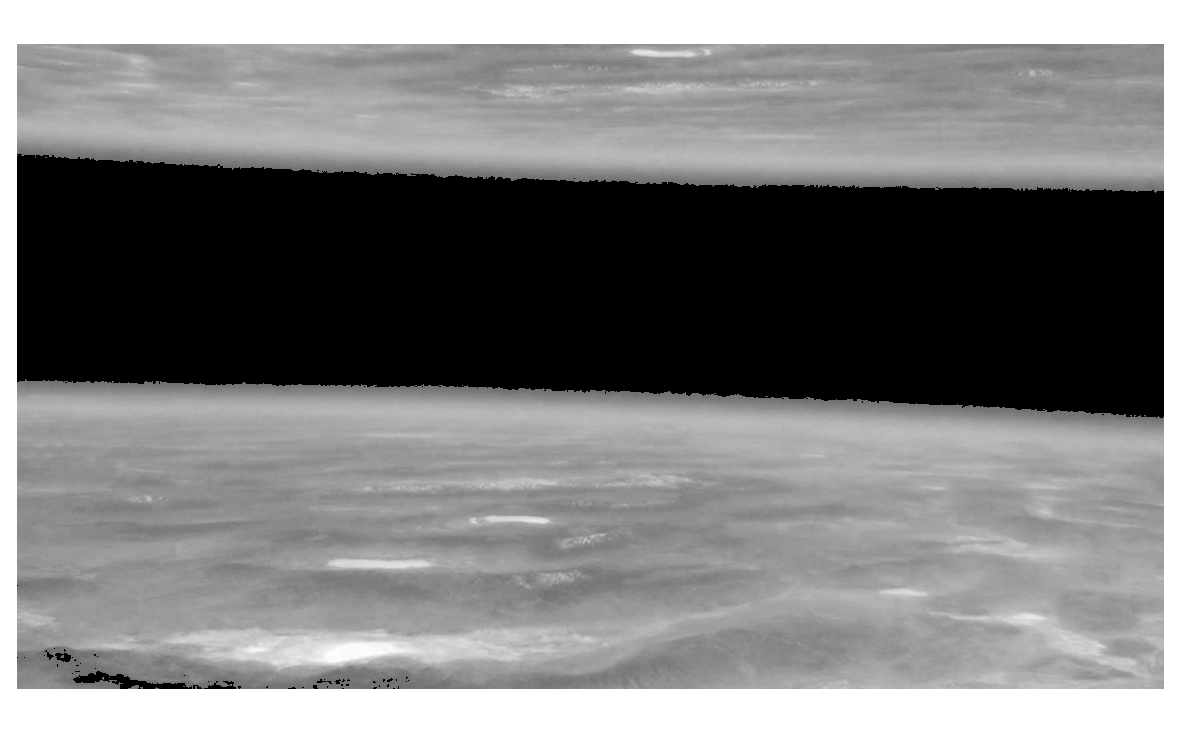
\includegraphics[width=.9\textwidth]{plots_tables_images/rmask.eps}
    \label{rmask}
\end{figure}

This image is misleading however, since the top and bottom profiles of the Earth should be symmetric about the X axis. To find the ``pitch'' of the camera, we mask the portion of the image that is space and find it's center of mass. Since the mask is symmetric around the X axis, the center of mass will find the Y position of the mask relative to the image. 

\begin{figure}[h]
        \begin{minipage}{.45\textwidth}
            % \begin{center}
            \centering
                
\includegraphics[width=\linewidth]{plots_tables_images/spacemask.eps}
                \caption{Mask of pixels not above the Earth-brightness threshold}
            % \end{center}
        \end{minipage}
        \hspace{.5in}
        \begin{minipage}{.45\textwidth}
            % \begin{center}
            \centering
                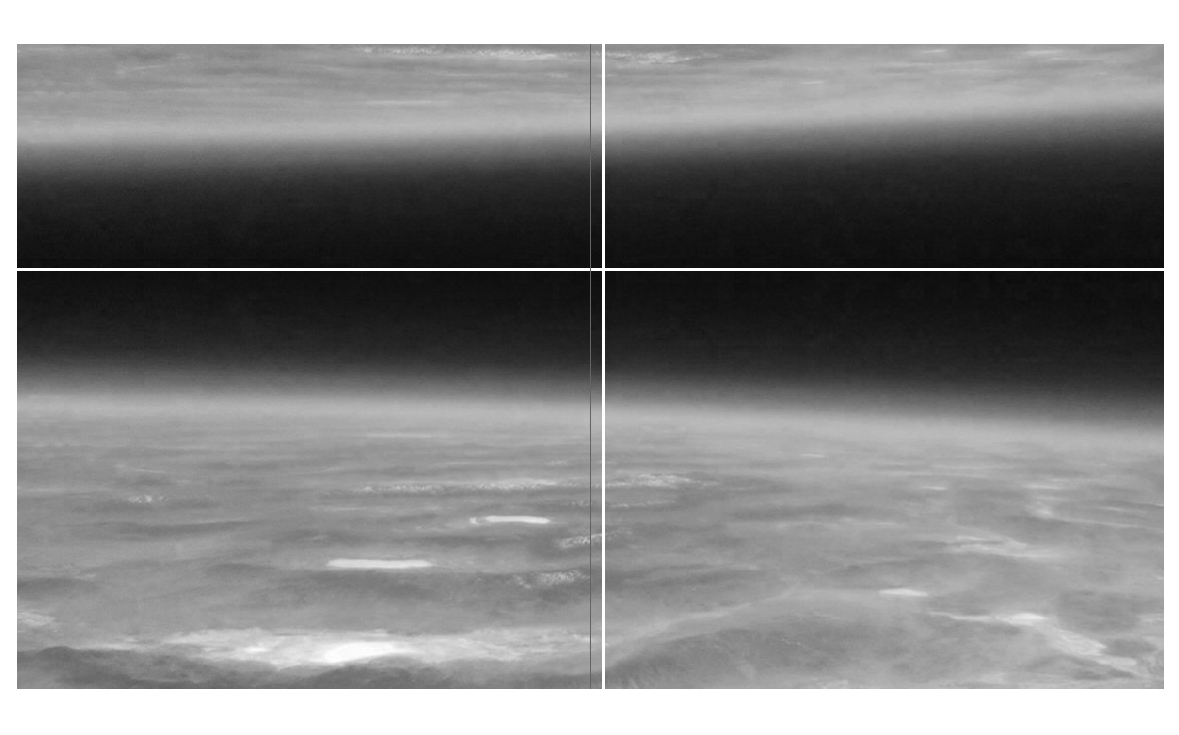
\includegraphics[width=\linewidth]{plots_tables_images/spreadc.eps}
                \caption{Center of mass of the space mask}
            % \end{center}
        \end{minipage}
    \end{figure}
% subsection pitch (end)

\subsection{``Roll''} % (fold)
\label{sub:roll}

To find ``roll'', we have to be a little more cautious. To begin with, we find the edges of the Earth in Figure \ref{raw} to get Figure \ref{earthlimb}.
% subsection roll (end)

\begin{figure}[!h]
    \centering
    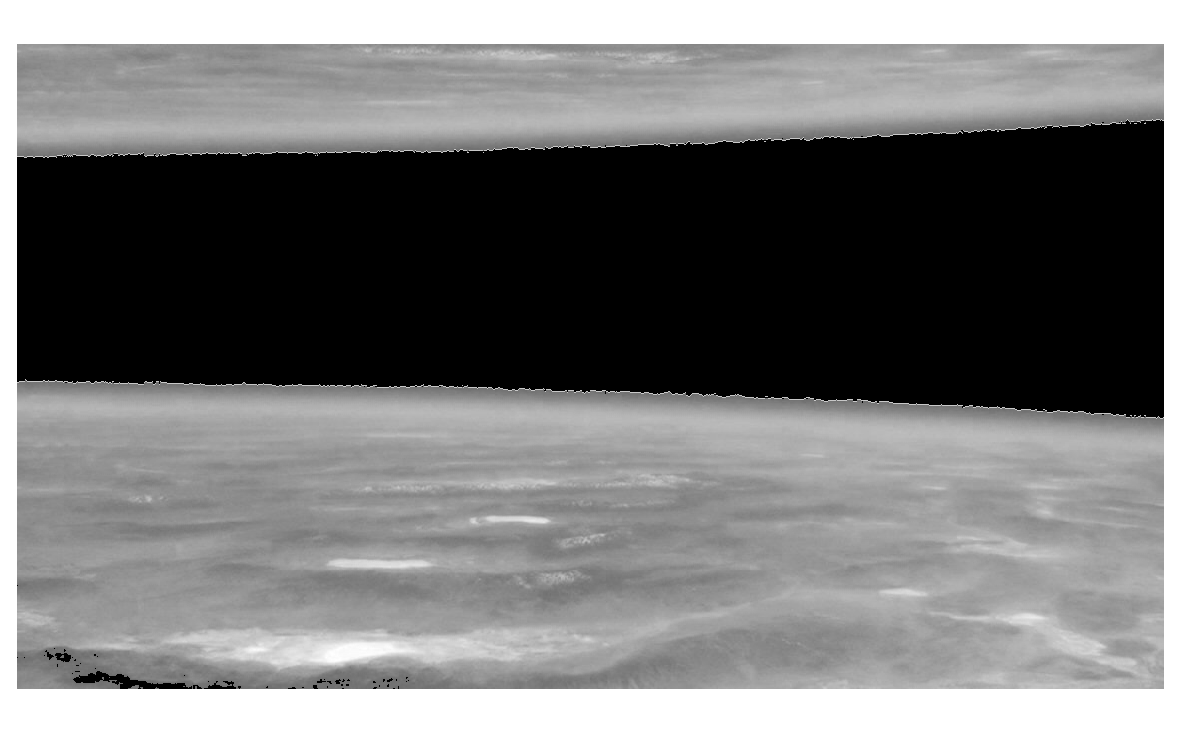
\includegraphics[width=.9\textwidth]{plots_tables_images/ama.eps}
    \label{earthlimb}
\end{figure}

We fit a 2nd order polynomial to the limb and record the height of the limb endpoints. 

\begin{figure}[!h]
    \centering
    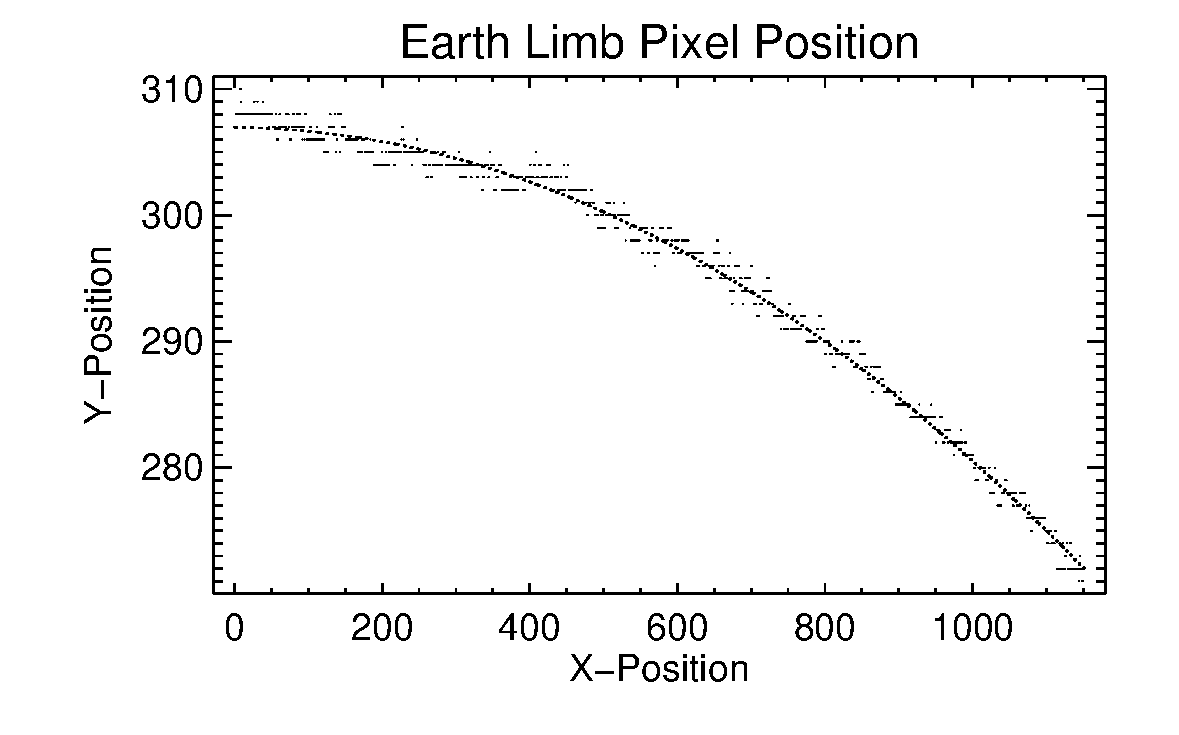
\includegraphics[width=.9\textwidth]{plots_tables_images/earth_limb.eps}
    \label{limbfit}
\end{figure}

With the endpoints, we can find the difference and take the tangent to find the angle the Earth appears to be rotated:

\begin{equation}
    \phi = \tan{ \left(\frac{ \textrm{difference in limb endpoint height} }{\textrm{width of image}} \right)}
\end{equation}

% section image_processing (end)

\section{Counting Pixels} % (fold)
\label{sec:counting_pixels}
One possibility of finding the angles is to count the pixels in each of the Earth masks and relate them to each other. However, I'm not sure if the loss/gain in each Earth profile is linear as we twist and turn the camera. If it is linear, then the pixel number lost in one mask should be gained in the other mask when rotating. However, if it's not linear, we have to find some coefficient and it gets a little harder. 

% section counting_pixels (end)

\section{Caveats} % (fold)
\label{sec:caveats}
I'll try to remake an image with an actual symmetrc earth limb and look into other alternatives to find the ``pitch'' and ``roll''. I use quotes because they are simply terms I've been using that don't hold any specific orientation or meaning.
% section caveats (end)










\end{document}